\documentclass[11pt,a4paper]{article}
\usepackage[utf8]{inputenc}
\usepackage[french]{babel}
\usepackage[T1]{fontenc}

\usepackage{amsmath}
\usepackage{amsfonts}
\usepackage{amssymb}

\newcommand{\NomAuteur}{Fabrice BOISSIER}
\newcommand{\TitreMatiere}{Architecture des Ordinateurs}
\newcommand{\NomUniv}{EPITA - Bachelor Cyber Sécurité}
\newcommand{\NiveauUniv}{CYBER1}
\newcommand{\NumGroupe}{CYBER1}
\newcommand{\AnneeUniv}{2024-2025}
\newcommand{\DateExam}{Novembre 2024}
\newcommand{\TypeExam}{CORRECTION Examen (Sujet B)}
\newcommand{\TitreExam}{\TitreMatiere}
\newcommand{\DureeExam}{1h30}
\newcommand{\MyWaterMark}{\AnneeUniv} % Watermark de protection

% Ajout de mes classes & definitions
\usepackage{MetalExam} % Appelle un .sty

% "Tableau" et pas "Table"
\addto\captionsfrench{\def\tablename{Tableau}}

%%%%%%%%%%%%%%%%%%%%%%%
%Header
%%%%%%%%%%%%%%%%%%%%%%%
\lhead{\TypeExam}							%Gauche Haut
\chead{\NomUniv}							%Centre Haut
\rhead{\NumGroupe}							%Droite Haut
\lfoot{\DateExam}							%Gauche Bas
\cfoot{\thepage{} / \pageref*{LastPage}}	%Centre Bas
\rfoot{\texttt{\TitreMatiere}}				%Droite Bas

%%%%%

\usepackage{tabularx}

\newlength{\LabelWidth}%
%\setlength{\LabelWidth}{1.3in}%
\setlength{\LabelWidth}{1cm}%
%\settowidth{\LabelWidth}{Employee E-mail:}%  Specify the widest text here.

% Optional first parameter here specifies the alignment of
% the text within the \makebox.  Default is [l] for left
% alignment. Other options are [r] and [c] for right and center
\newcommand*{\AdjustSize}[2][l]{\makebox[\LabelWidth][#1]{#2}}%


\definecolor{mGreen}{rgb}{0,0.6,0}
\definecolor{mGray}{rgb}{0.5,0.5,0.5}
\definecolor{mPurple}{rgb}{0.58,0,0.82}
\definecolor{backgroundColour}{rgb}{0.95,0.95,0.92}

\lstdefinestyle{CStyle}{
    backgroundcolor=\color{backgroundColour},
    commentstyle=\color{mGreen},
    keywordstyle=\color{magenta},
    numberstyle=\tiny\color{mGray},
    stringstyle=\color{mPurple},
    basicstyle=\footnotesize,
    breakatwhitespace=false,
    breaklines=true,
    captionpos=b,
    keepspaces=true,
    numbers=left,
    numbersep=5pt,
    showspaces=false,
    showstringspaces=false,
    showtabs=false,
    tabsize=2,
    language=C
}


\hyphenation{op-tical net-works SIGKILL}


\begin{document}

%\MakeExamTitleDuree     % Pour afficher la duree
\MakeExamTitle                   % Ne pas afficher la duree

%% \MakeStudentName    %% A reutiliser sur chaque nouvelle page

\bigskip
%\bigskip

Vous devez respecter les consignes suivantes, sous peine de 0 :

\begin{itemize}
\item Lisez le sujet en entier avec attention
\item Répondez sur le sujet
\item Ne détachez pas les agrafes du sujet
\item \'Ecrivez lisiblement vos réponses (si nécessaire en majuscules)
\item Les appareils électroniques sont tous interdits (calculatrices également)
\item Ne trichez pas
\end{itemize}

%\bigskip

\vfillFirst

% Questions cours
\section{Questions (14 points)}

\subsection{(2 points) Rappelez les 14 premières puissances de 2 : }

\bigskip


\begin{table}[ht!]
\centerline{
\begin{tabular}{ | m{0.5cm} | m{0.5cm} | m{0.5cm} | m{0.5cm} | m{0.65cm} | m{0.65cm} | m{0.65cm} | m{1cm} | m{1cm} | m{1cm} | m{1.5cm} | m{1.5cm} | m{1.5cm} | m{1.5cm} |}
\hline
$ 2^{0} $ & $ 2^{1} $ & $ 2^{2} $ & $ 2^{3} $ & $ 2^{4} $ & $ 2^{5} $ & $ 2^{6} $ & $ 2^{7} $ & $ 2^{8} $ & $ 2^{9} $ & $ 2^{10} $ & $ 2^{11} $ &  $ 2^{12} $ &  $ 2^{13} $ \\
\hline
1 & 2 & 4 & 8 & 16 & 32 & 64 & 128 & 256 & 512 & 1024 & 2048 & 4096 & 8192 \\
\hline
\end{tabular}
}
\end{table}


\bigskip

\subsection{(4 points) Convertissez ces nombres binaires en décimaux. Vous donnerez leur interprétation sur 12 bits en tant que nombre signé, puis non-signé.}

\bigskip

\centerline{
\begin{tabular}{ c ||  C{5cm} || C{5cm} }
 & \multirow{3}{*}[0pt]{signé}
 & \multirow{3}{*}[0pt]{non-signé}
 \\
%
 & & \\
 & & \\
%
\hline
\multirow{3}{*}[0pt]{ $ \% \, 0111 \; 1101 \; 1100 $ } & \multirow{3}{*}[0pt]{ $ 2012 $ } & \multirow{3}{*}[0pt]{ $ 2012 $ } \\
 & & \\
 & & \\
\hline
\multirow{3}{*}[0pt]{ $ \% \, 1100 \; 0011 \; 0110 $ } & \multirow{3}{*}[0pt]{ $ -970 $ } & \multirow{3}{*}[0pt]{ $ 3126 $ } \\
 & & \\
 & & \\
\hline
\multirow{3}{*}[0pt]{ \$ 7BD } & \multirow{3}{*}[0pt]{ $ 1981 $ } & \multirow{3}{*}[0pt]{ $ 1981 $ } \\
 & & \\
 & & \\
\hline
\multirow{3}{*}[0pt]{ \$ 9CD } & \multirow{3}{*}[0pt]{ $ -1587 $ } & \multirow{3}{*}[0pt]{ $ 2509 $ } \\
 & & \\
 & & \\
\end{tabular}
}

\bigskip


\vfillLast

\clearpage


\subsection{(3 points) Convertissez ces nombres décimaux en binaire sur 12 bits, puis en hexadécimal.}

\bigskip

\centerline{
\begin{tabular}{ | c |C{0.33cm}|C{0.33cm}|C{0.33cm}|C{0.33cm}||C{0.33cm}|C{0.33cm}|C{0.33cm}|C{0.33cm}||C{0.33cm}|C{0.33cm}|C{0.33cm}|C{0.33cm}| c | }
\hline
                         & \multicolumn{12}{c|}{binaire} & \multicolumn{1}{c|}{hexadécimal} \\
\hline

\multirow[c]{2}{*}[0in]{42}   &    & & & & & & & & & & &    & \multirow[c]{2}{*}[0in]{ \$ 02A } \\
                              &   0 & 0 & 0 & 0 & 0 & 0 & 1 & 0 & 1 & 0 & 1 & 0   & \\
\hline

\multirow[c]{2}{*}[0in]{2138} &    & & & & & & & & & & &    & \multirow[c]{2}{*}[0in]{ \$ 85A } \\
                              &   1 & 0 & 0 & 0 & 0 & 1 & 0 & 1 & 1 & 0 & 1 & 0   & \\
\hline

\multirow[c]{2}{*}[0in]{-628} &    & & & & & & & & & & &    & \multirow[c]{2}{*}[0in]{ \$ D8C } \\
                              &   1 & 1 & 0 & 1 & 1 & 0 & 0 & 0 & 1 & 1 & 0 & 0   & \\
\hline
\end{tabular}
}

\bigskip


\bigskip


% Gray / BCD
\subsection{(2 points) Convertissez ces nombres décimaux en code Gray sur 12 bits : }

\bigskip

\centerline{
\begin{tabular}{ | c |C{0.33cm}|C{0.33cm}|C{0.33cm}|C{0.33cm}||C{0.33cm}|C{0.33cm}|C{0.33cm}|C{0.33cm}||C{0.33cm}|C{0.33cm}|C{0.33cm}|C{0.33cm}| }
\hline
                         & \multicolumn{12}{c|}{binaire Gray} \\ % Gray / BCD
\hline

\multirow[c]{2}{*}[0in]{42}   &    & & & & & & & & & & & \\
                              &   0 & 0 & 0 & 0 & 0 & 0 & 1 & 1 & 1 & 1 & 1 & 1 \\
\hline

\multirow[c]{2}{*}[0in]{2138} &    & & & & & & & & & & & \\
                              &   1 & 1 & 0 & 0 & 0 & 1 & 1 & 1 & 0 & 1 & 1 & 1 \\
\hline
\end{tabular}
}

\bigskip

\bigskip


\subsection{(3 points) Effectuez les opérations suivantes : }

\bigskip

\centerline{
\begin{tabular}{ | c |C{0.33cm}|C{0.33cm}|C{0.33cm}|C{0.33cm}||C{0.33cm}|C{0.33cm}|C{0.33cm}|C{0.33cm}||C{0.33cm}|C{0.33cm}|C{0.33cm}|C{0.33cm}| }
\hline
Opérations & \multicolumn{12}{c|}{Résultats} \\
\hline
\multirow[c]{2}{*}[0in]{ $ \% \, 0111 \; 1001 \; 1110
               \;\; + \;\; \% \, 0010 \; 1011 \; 0111 $ }  % 1950 + 695 = 2645
 &    & & & & & & & & & & & \\
 &   1 & 0 & 1 & 0 & 0 & 1 & 0 & 1 & 0 & 1 & 0 & 1 \\
\hline
\multirow[c]{2}{*}[0in]{ $ \% \, 1111 \; 1101 \; 1110
               \;\; - \;\; \% \, 0110 \; 1011 \; 0100 $ }  % 4062 - 1716 = 2346
 &    & & & & & & & & & & & \\
 &   1 & 0 & 0 & 1 & 0 & 0 & 1 & 0 & 1 & 0 & 1 & 0 \\
\hline
\multirow[c]{2}{*}[0in]{ $ \% \, 1101 \; 0110 \;\; \times \;\; \% \, 0110 $ }  % 214 * 6 = 1284
 &    & & & & & & & & & & & \\
 &   0 & 1 & 0 & 1 & 0 & 0 & 0 & 0 & 0 & 1 & 0 & 0 \\
\hline
\end{tabular}
}


\bigskip

\bigskip


%\subsection{(2 points) Convertissez ces nombres flottants vers le format IEEE 754 simple précision : }
%
%\bigskip
%
%\centerline{
%\begin{tabular}{| c ||  c |C{0.33cm}|C{0.33cm}|C{0.33cm}|C{0.33cm}|C{0.33cm}|C{0.33cm}|C{0.33cm}|C{0.33cm}   ||  c |C{0.33cm}|C{0.33cm}|C{0.33cm}|C{0.33cm}|C{0.33cm}|C{0.33cm}|%C{0.33cm}|C{0.33cm}|C{0.33cm}| }
%\hline
%                                          & \multicolumn{9}{c||}{\multirow{2}{*}{exposant}}   & \multicolumn{9}{c|}{\multirow{2}{*}{hexadécimal}} \\
%                                          & \multicolumn{9}{c||}{ }                           & \multicolumn{9}{c|}{ } \\
%\hline
%\multirow[c]{3}{*}[0in]{$ 68,78125 $}     & \multirow[c]{3}{*}[0in]{$ \% $} & & & & & & & &  & \multirow[c]{3}{*}[0in]{$ \$ $} & & & & & & & & \\
%                                          & & & & & & & & &                                  & & & & & & & & & \\
%                                          & & & & & & & & &                                  & & & & & & & & & \\
%\hline
%\multirow[c]{3}{*}[0in]{$ -218,3203125 $} & \multirow[c]{3}{*}[0in]{$ \% $} & & & & & & & &  & \multirow[c]{3}{*}[0in]{$ \$ $} & & & & & & & & \\
%                                          & & & & & & & & &                                  & & & & & & & & & \\
%                                          & & & & & & & & &                                  & & & & & & & & & \\
%\hline
%\end{tabular}
%}
%
%\bigskip
%\bigskip

\bigskip


\vfillFirst

%\begin{center}
%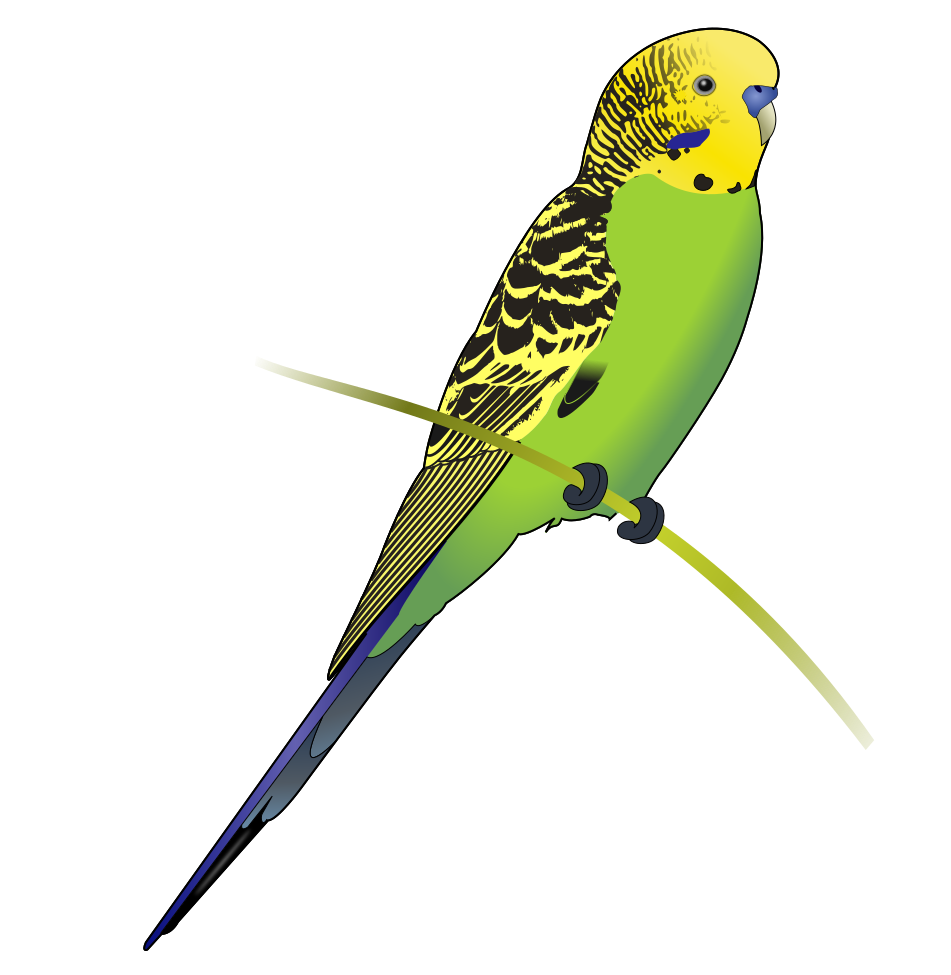
\includegraphics[scale=0.2]{img/others/Budgerigar_diagram.png}
%\end{center}

\vfillLast

\clearpage

%%%%%%%%%%%%%%%%%%%%%%%%%%%%%%%%%%%%%%%%%%%%%%%%%%%%%%%
%%%%%%%%%%%%%%%%%%%%%%%%%%%%%%%%%%%%%%%%%%%%%%%%%%%%%%%
%%%%%%%%%%%%%%%%%%%%%%%%%%%%%%%%%%%%%%%%%%%%%%%%%%%%%%%

\section{ASCII (6 points)}

\noindent Vous avez maintenant compris qu'une donnée brute peut être interprétée de plusieurs façons possibles : en tant qu'entier signé ou entier non-signé, voire qu'il s'agit d'une valeur en code Gray ou en BCD.
Néanmoins, il existe de nombreux autres formats de données !

\noindent Parmi tous ces formats, il existe le célèbre code ASCII permettant de représenter les caractères simples de l'alphabet latin (les lettres en majuscules, en minuscules, les chiffres, la ponctuation, ainsi que des caractères dédiées aux machines comme le retour à la ligne).

\medskip

\noindent Vous allez donc maintenant transformer un bloc de données issu d'un fichier texte brut en ASCII (donc récupéré de la mémoire d'un ordinateur) en un texte lisible par un humain.
Notez bien qu'un caractère utilise exactement 1 octet, c'est-à-dire 8 bits.

\bigskip

\noindent Pour vous aider à retrouver les chaînes de caractères, une table ASCII décimale/caractères est fournie :

\begin{center}
\begin{tabular}{ | l |c|c|c|c|c| c |c|c|c|c|c|c|c|c|c|c| }
\hline
Char & \textbackslash{}n & \textbackslash{}r & \textit{(espace)} &  - &  . &   & 0 &  1 &  2 &  3 &  4 &  5 &  6 &  7 &  8 &  9 \\
\hline
Dec &         10         &        13         &         32        & 45 & 46 &   & 48 & 49 & 50 & 51 & 52 & 53 & 54 & 55 & 56 & 57 \\
\hline
\end{tabular}
%\end{center}

%\bigskip
\medskip

%\begin{center}
%\centerline{
%\begin{tabular}{ | l |c|c|c|c|c|c|c|c|c|c|c|c|c|c|c|c|c|c|c|c|c|c|c|c|c|c| }
%\hline
%Char &  A &  B &  C &  D &  E &  F &  G &  H &  I &  J &  K &  L &  M &  N &  O &  P &  Q &  R &  S &  T &  U &  V &  W &  X &  Y &  Z \\
%\hline
%Dec &  65 & 66 & 67 & 68 & 69 & 70 & 71 & 72 & 73 & 74 & 75 & 76 & 77 & 78 & 79 & 80 & 81 & 82 & 83 & 84 & 85 & 86 & 87 & 88 & 89 & 90 \\
%\hline
%\end{tabular}

\begin{tabular}{ | l |c|c|c|c|c|c|c|c|c|c|c|c|c| }
\hline
Char &  A &  B &  C &  D &  E &  F &  G &  H &  I &  J &  K &  L &  M \\
\hline
Dec &  65 & 66 & 67 & 68 & 69 & 70 & 71 & 72 & 73 & 74 & 75 & 76 & 77 \\
\hline
%\end{tabular}
%
%\smallskip
%
%\begin{tabular}{ | l |c|c|c|c|c|c|c|c|c|c|c|c|c| }
\hline
Char &  N &  O &  P &  Q &  R &  S &  T &  U &  V &  W &  X &  Y &  Z \\
\hline
Dec &  78 & 79 & 80 & 81 & 82 & 83 & 84 & 85 & 86 & 87 & 88 & 89 & 90 \\
\hline
\end{tabular}

%}

%\bigskip
\medskip

\begin{tabular}{ | l |c|c|c|c|c|c|c|c|c|c|c|c|c| }
\hline
Char &  a &  b &  c &  d  &  e  &  f  &  g  &  h  &  i  &  j  &  k  &  l  &  m \\
\hline
Dec &  97 & 98 & 99 & 100 & 101 & 102 & 103 & 104 & 105 & 106 & 107 & 108 & 109 \\
\hline
%\end{tabular}
%
%\smallskip
%
%\begin{tabular}{ | l |c|c|c|c|c|c|c|c|c|c|c|c|c| }
\hline
Dec &  110 & 111 & 112 & 113 & 114 & 115 & 116 & 117 & 118 & 119 & 120 & 121 & 122 \\
\hline
Char &  n  &  o  &  p  &  q  &  r  &  s  &  t  &  u  &  v  &  w  &  x  &  y  &  z \\
\hline
\end{tabular}

\end{center}

%\smallskip
%\medskip
%\newpage

%Le disque dur que l'on veut récupérer a apparemment été formaté en FAT12, c'est-à-dire que les fichiers ont un nom dont la taille est très limitée (8 caractères avant l'extension, et 3 après).

\bigskip

\begin{table}[h!]
  \centering
  \begin{minipage}{0.45\textwidth}

\subsection{(1 point) Préparation }

\smallskip

\noindent Avant de démarrer, commencez par convertir la valeur hexadécimale \TTBF{44} en décimal, afin de retrouver le caractère associé.

  \end{minipage}
  \hfillx
  \begin{minipage}{0.45\textwidth}
    \centering

\begin{center}
\begin{tabular}{ | l | C{1cm} | }
\hline
\multirow[c]{2}{*}[0in]{Caractères}  & \multirow[c]{2}{*}[0in]{D} \\
 & \\
\hline
\multirow[c]{2}{*}[0in]{Décimal}     & \multirow[c]{2}{*}[0in]{68} \\
 & \\
\hline
\multirow[c]{2}{*}[0in]{Hexadécimal} & \multirow[c]{2}{*}[0in]{44} \\
 & \\
\hline
\end{tabular}
\end{center}

  \end{minipage}
\end{table}


%\smallskip


\subsection{(5 points) Bloc de données }

\smallskip

\noindent Maintenant que vous avez compris la démarche, décodez le texte ci-dessous en respectant bien les majuscules et minuscules :

%\medskip

\begin{table}[ht!]
  \centering
%  \hspace*{-1.1cm}
  \begin{minipage}{0.4\textwidth}
    \centering
% %*   *)
\begin{lstlisting}[style=algorithmique]
44 65 73 73 69 6E 65 7A
20 64 65 73 20 44 69 6E
6F 73 61 75 72 65 73 2E
43 20 65 73 74 20 63 68
6F 75 65 74 74 65 00 00
\end{lstlisting}
  \end{minipage}
  \hfillx
  \begin{minipage}{0.45\textwidth}
    \centering

\begin{tabular}{ | m{0.45cm} | m{0.45cm} | m{0.45cm} | m{0.45cm}   |   m{0.45cm} | m{0.45cm} | m{0.45cm} | m{0.45cm} | }
\hline
   &   &   &   &   &   &   &   \\
 D & e & s & s & i & n & e & z \\
\hline
   &   &   &   &   &   &   &   \\
   & d & e & s &   & D & i & n \\
\hline
   &   &   &   &   &   &   &   \\
 o & s & a & u & r & e & s & . \\
\hline
   &   &   &   &   &   &   &   \\
 C &   & e & s & t &   & c & h \\
\hline
   &   &   &   &   &   &   &   \\
 o & u & e & t & t & e &   &   \\
\hline
\end{tabular}

  \end{minipage}
%  \caption{Algorithme de la somme des N premiers entiers}
%  \label{somme-n-premiers-entiers}
\end{table}

%%%%%%%%%%%%%%%%%%%%%%%%%%%%%%%%%%%%%%%%%%%%%%%%%%%%%%%%%%%%%%%%%%%%%%%%%%%%%

%\vfillFirst
%
%\begin{center}
%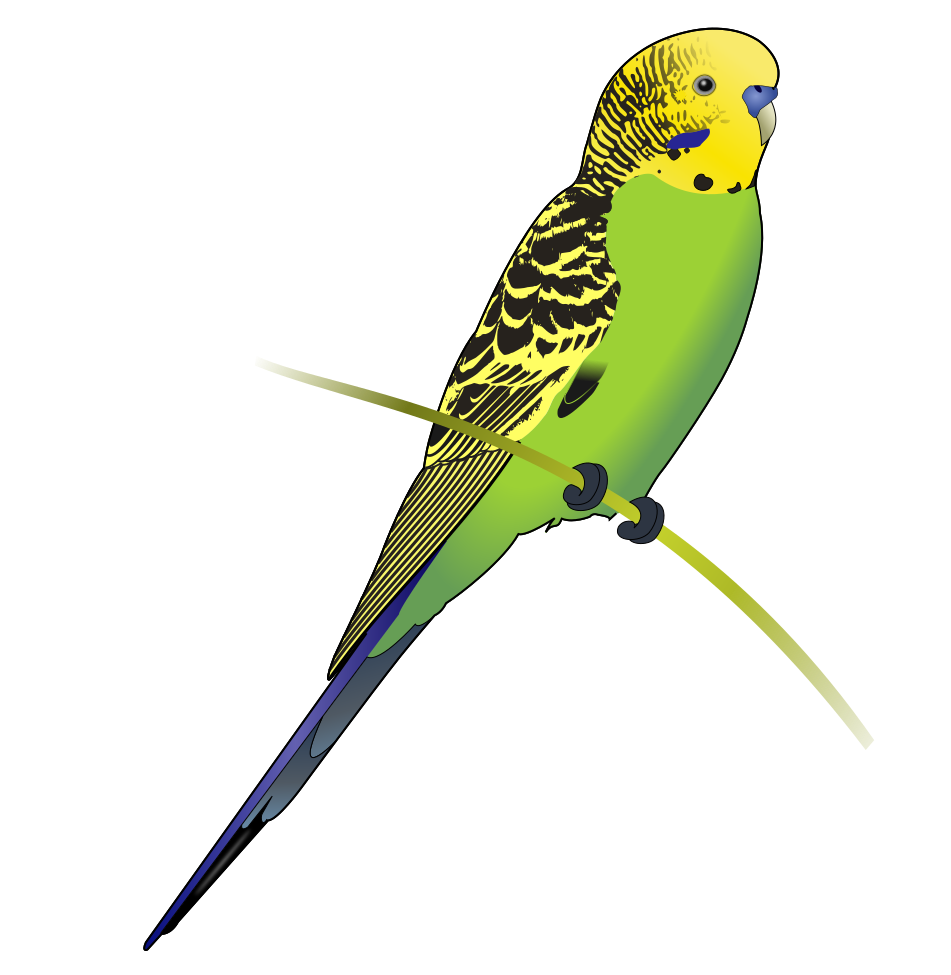
\includegraphics[scale=0.2]{img/others/Budgerigar_diagram.png}
%\end{center}
%
%\vfillLast

\newpage


%\thispagestyle{empty}

\vfillFirst

\begin{center}

\begin{LARGE}
\textbf{SUJET B CORRECTION}

\bigskip

\textbf{\MakeUppercase{\TitreMatiere}}
\end{LARGE}

\end{center}

\vfillLast

\end{document}
